\documentclass[10.5pt]{jsarticle}
\usepackage[hiresbb]{graphicx}
\usepackage{color}
\usepackage{amsmath,amssymb}
\usepackage{here}

\begin{document}
\section{判別基準評価}
\subsection{(a)}
  Nearest Neighbor、ユークリッド距離、類似度および重みつきユークリッド距離法(重み:(1,5))を用いてテストデータAを判別し,
  その認識正誤表と認識率を表1に示す.
  \begin{table}[htb]
    \caption{方法別認識正誤表}
    \begin{tabular}{|c||c|c|} \hline
      方法 & 正誤 & 認識率[\%] \\ \hline
      Nearest & TTTTTTTTTTFTTTTTTFTFTTFTTFTTTTTTTTTTTFFF & 80.0 \\\hline
      ユークリッド距離 & TFTTTTTTTTTTTFTTFFTFTTTTTTTTTFTFTTFTTFTT & 77.5 \\\hline
      重み付きユークリッド & TFTTTTTTTTTTTFTTFFTFTTTTTTTTTFTFTTFTTFTT & 77.5\\\hline
      類似度 & TFTTTTTTTTTTTFTTFFTFTTTTTTTTTFTFTTFTTFTT & 77.5\\\hline
    \end{tabular}
  \end{table}

\subsection{(b)}
  次に, それぞれの方法で識別した散布図, 学習データ平均と識別境界線を一つにまとめた結果図を順に図1(a)-(e)に示す.\\\\\\\\

\begin{figure}[hbtp]
  \centering
  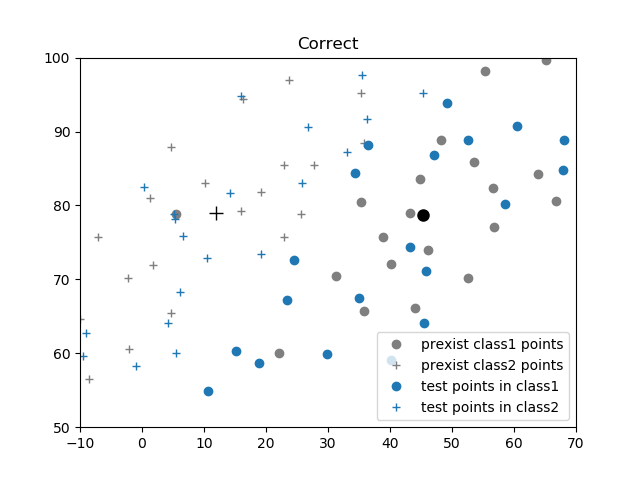
\includegraphics[width=22.1cm, bb=9 9 700 270]{results/CorrectResultFigureA.png}
  \caption{(a) Correct distribution of test set A.}
\end{figure}

\begin{figure}[htbp]
  \centering
  \begin{tabular}{c}
  	\begin{minipage}{0.56\hsize}
  	\centering
  		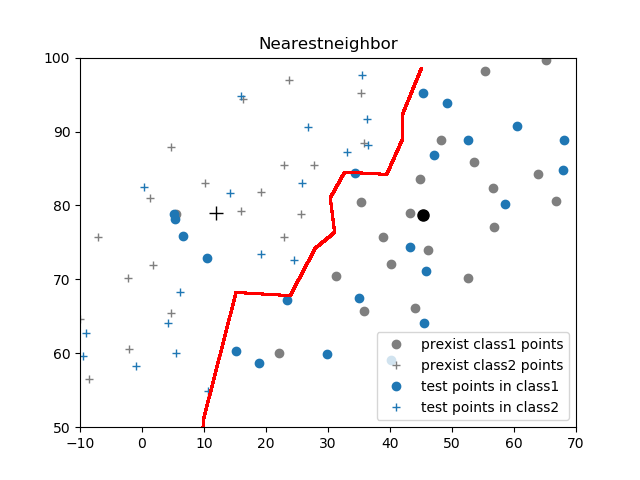
\includegraphics[width=15.0cm, bb=9 9 700 270]{results/NearestneighborResultFigureA.png}
  		\hspace{0cm} (b) The result of using Nearest Neighbor method.
  	\end{minipage}

  	\begin{minipage}{0.5\hsize}
  	\centering
  		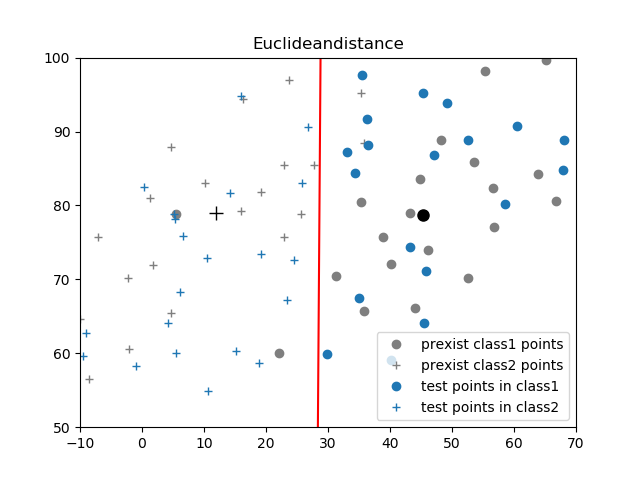
\includegraphics[width=15.0cm, bb=9 9 700 270]{results/EuclideandistanceResultFigureA.png}
  		\hspace{0cm} (b) The result of using EuclideanDistance method.
  	\end{minipage}
  \end{tabular}
\end{figure}
.\\
\begin{figure}[htbp]
  \centering
  \begin{tabular}{c}
  	\begin{minipage}{0.56\hsize}
  	\centering
  		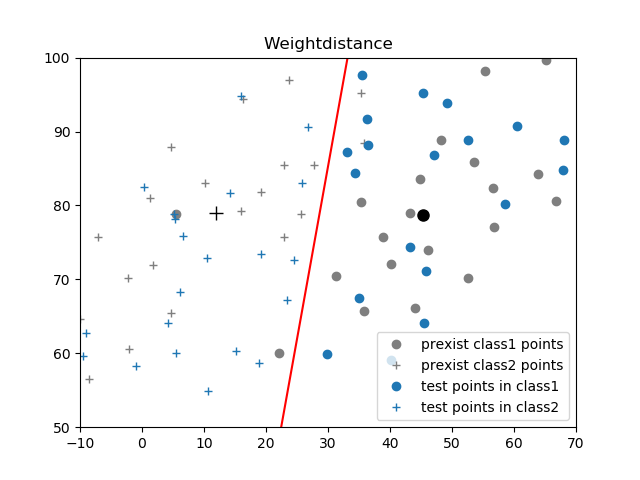
\includegraphics[width=15.0cm, bb=9 9 700 270]{results/WeightdistanceResultFigureA.png}
  		\hspace{0cm} (d) The result of using Weight Euclidean method.
  	\end{minipage}

  	\begin{minipage}{0.5\hsize}
  	\centering
  		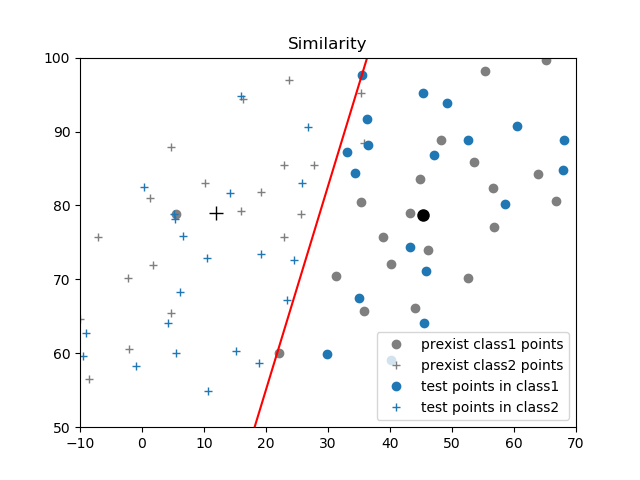
\includegraphics[width=15.0cm, bb=9 9 700 270]{results/SimilarityResultFigureA.png}
  		\hspace{0cm} (e) The result of using Similarity method.
  	\end{minipage}
  \end{tabular}
\end{figure}

上図から, Nearest Neighbor法はノイズに弱く, class2の群れの中にclass1点が一つあるだけでその周りにいる未知点がclass1に判定されてしまう.
ユークリッド距離法では各クラス平均の分布状況によって判別基準が大きく左右されることがあることがわかった. 例えば, 図1(c)に示したように,
今回の学習データAのclass1とclass2の平均点(それぞれ大きい黒丸と大きい黒プラス記号で表した)の{\bf y座標がほぼ変わらず}, 識別境界線も
自明にその中心を結んだものと垂直な線になり, テストデータはほぼ各点のx座標で分類されたことがわかった.\\
この問題を改善すべく現れたのが重み付きユークリッド距離法である. 図1(c)で示したように, この方法ではそれぞれの軸に重みをかけることができ,
今回の学習データAに対しては平均点がほぼx軸に平行な直線上に分布していることを考慮し, 各テストデータのy座標の影響を引き出すためにx軸に1, y軸に2
の重みをかけた. 類似度判別では, 原点からの角度で判別状況が大きく変わるため, テストデータの分布状況は認識率に大きな影響を与えることが
予想できる.

\subsection{(c) - データセットB}
データセットB, C, Dについても上記と同じように分析し結果を下表2-4及び図2-4に示した.

\begin{table}[htbp]
  \caption{方法別認識正誤表(B)}
  \begin{tabular}{|c||c|c|} \hline
    方法 & 正誤 & 認識率[\%] \\ \hline
    Nearest & TTTTTTTTTTFTTTTTTTTTTTTFTTTTTTTTTTTTTTT & 95.0 \\\hline
    ユークリッド距離 & TTTTTTTTTTFTFTTTTFTTTTTTTTTTTTTTTTTTTFT & 90.0 \\\hline
    重み付きユークリッド & FTTFTTFTTTFTTTFTTTFTTTTFFTTFTTTTTFTFFTTT & 70.0\\\hline
    類似度 & TFTTTTTTTTFTFFTTFFTFFTTTTTTTTFTFTTFTTFTT & 70.0\\\hline
  \end{tabular}
\end{table}

\begin{figure}[hbtp]
  \centering
  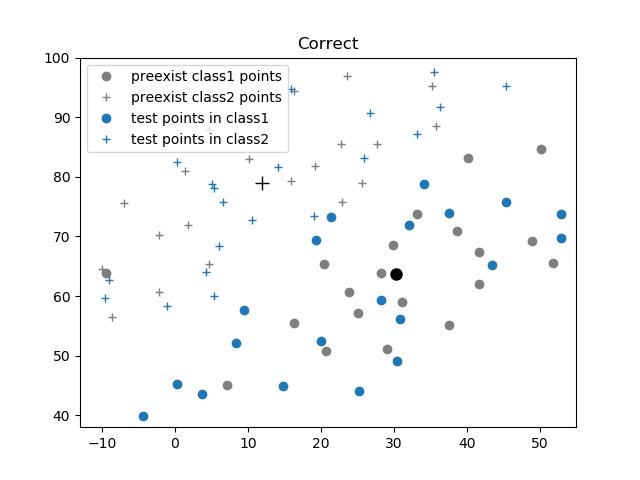
\includegraphics[width=26cm, bb=9 9 700 350]{results/CorrectResultFigureB.png}
  \caption{(a) Correct distribution of test set B.}
\end{figure}

\begin{figure}[htbp]
  \centering
  \begin{tabular}{c}
  	\begin{minipage}{0.56\hsize}
  	\centering
  		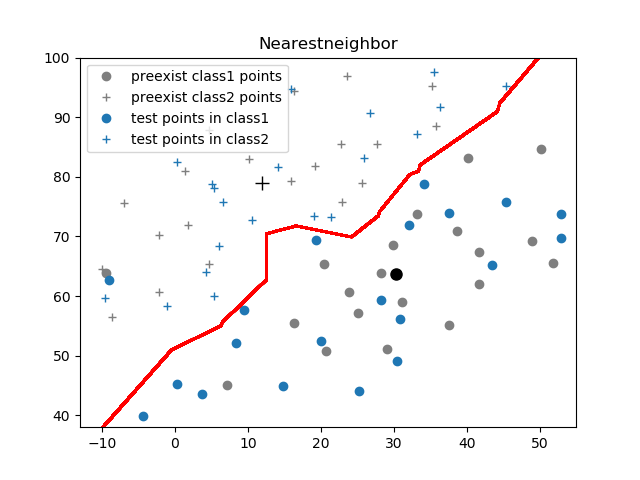
\includegraphics[width=15.0cm, bb=9 9 700 270]{results/NearestneighborResultFigureB.png}
  		\hspace{0cm} (b) The result of using Nearest Neighbor method. (B)
  	\end{minipage}

  	\begin{minipage}{0.5\hsize}
  	\centering
  		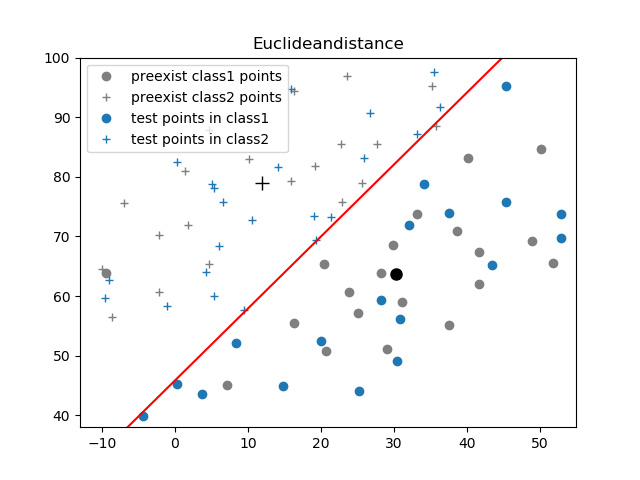
\includegraphics[width=15.0cm, bb=9 9 700 270]{results/EuclideandistanceResultFigureB.png}
  		\hspace{0cm} (b) The result of using EuclideanDistance method.
  	\end{minipage}
  \end{tabular}
\end{figure}
\begin{figure}[htbp]
  \centering
  \begin{tabular}{c}
  	\begin{minipage}{0.56\hsize}
  	\centering
  		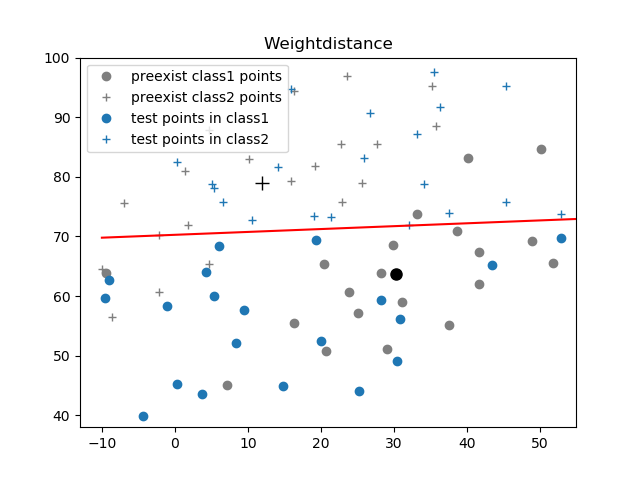
\includegraphics[width=15.0cm, bb=9 9 700 270]{results/WeightdistanceResultFigureB.png}
  		\hspace{0cm} (d) The result of using Weight Euclidean method. (B)
  	\end{minipage}

  	\begin{minipage}{0.5\hsize}
  	\centering
  		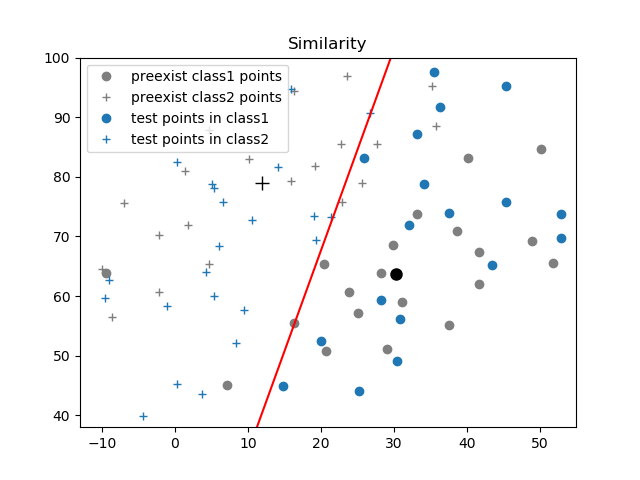
\includegraphics[width=15.0cm, bb=9 9 700 270]{results/SimilarityResultFigureB.png}
  		\hspace{0cm} (e) The result of using Similarity method. (B)
  	\end{minipage}
  \end{tabular}
\end{figure}


\clearpage
\setcounter{subsection}{1}
\subsection{データセットC}

\begin{table}[htbp]
  \caption{方法別認識正誤表(C)}
  \begin{tabular}{|c||c|c|} \hline
    方法 & 正誤 & 認識率[\%] \\ \hline
    Nearest & TTTTTTTTTTFTTTTTTFTFTTFTTFTTTTTTTTTTTFFF & 80.0 \\\hline
    ユークリッド距離 & TFTTTTTTTTTTTFTTFFTFTTTTTTTTTFTFTTFTTFTT & 77.5 \\\hline
    重み付きユークリッド & TFTTTTTTTTTTTFTTFFTFTTTTTTTTTFTFTTFTTFTT & 77.5\\\hline
    類似度 & TTTTTTTTTTTTTTTTTTTTTTTTTTTTTFTFTTTTTFTT & 92.5\\\hline
  \end{tabular}
\end{table}

 \begin{figure}[hbtp]
   \centering
   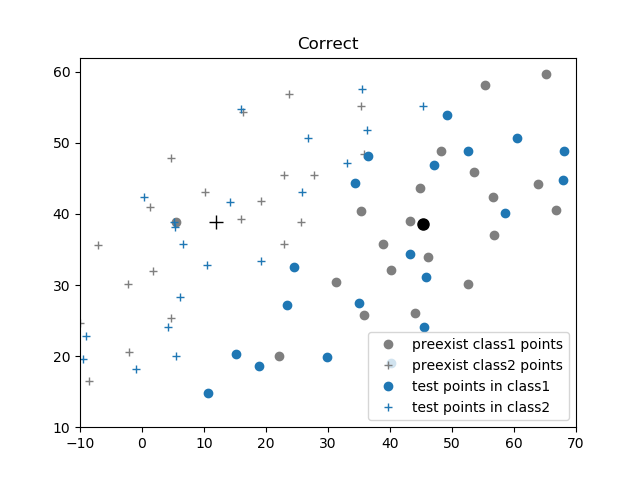
\includegraphics[width=26cm, bb=9 9 700 350]{results/CorrectResultFigureC.png}
   \caption{(a) Correct distribution of test set C.}
 \end{figure}

 \begin{figure}[htbp]
   \centering
   \begin{tabular}{c}
   	\begin{minipage}{0.56\hsize}
   	\centering
   		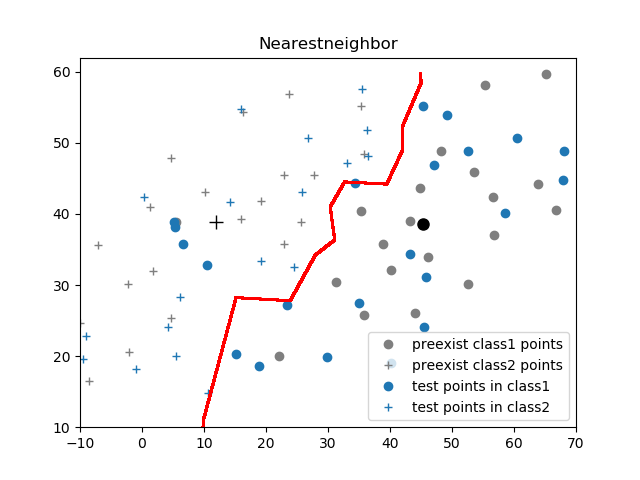
\includegraphics[width=15.0cm, bb=9 9 700 270]{results/NearestneighborResultFigureC.png}
   		\hspace{0cm} (b) The result of using Nearest Neighbor method. (C)
   	\end{minipage}

   	\begin{minipage}{0.5\hsize}
   	\centering
   		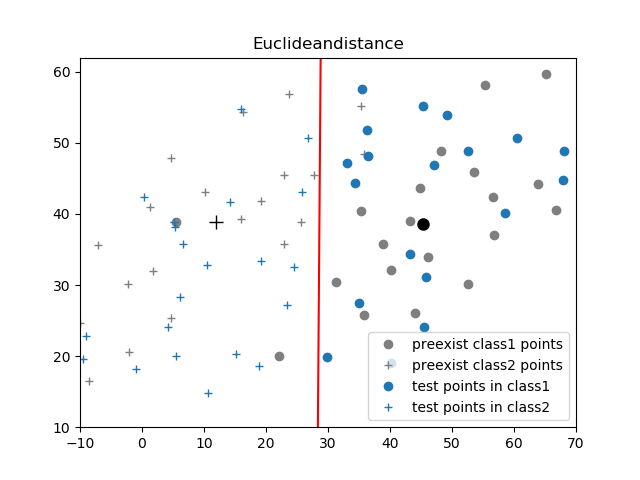
\includegraphics[width=15.0cm, bb=9 9 700 270]{results/EuclideandistanceResultFigureC.png}
   		\hspace{0cm} (b) The result of using EuclideanDistance method.
   	\end{minipage}
   \end{tabular}
 \end{figure}
 \begin{figure}[htbp]
   \centering
   \begin{tabular}{c}
   	\begin{minipage}{0.56\hsize}
   	\centering
   		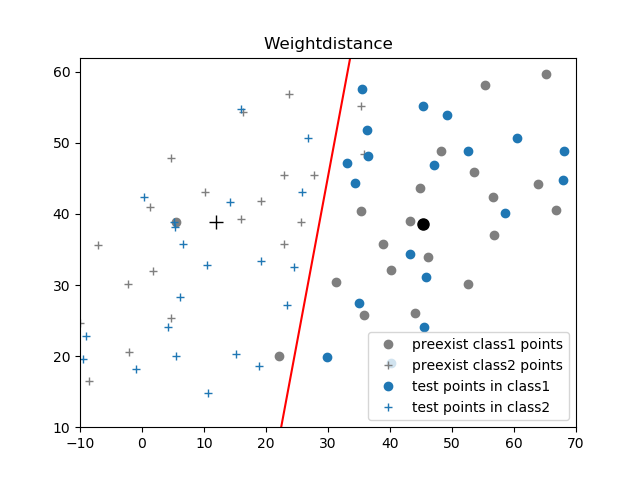
\includegraphics[width=15.0cm, bb=9 9 700 270]{results/WeightdistanceResultFigureC.png}
   		\hspace{0cm} (d) The result of using Weight Euclidean method. (C)
   	\end{minipage}

   	\begin{minipage}{0.5\hsize}
   	\centering
   		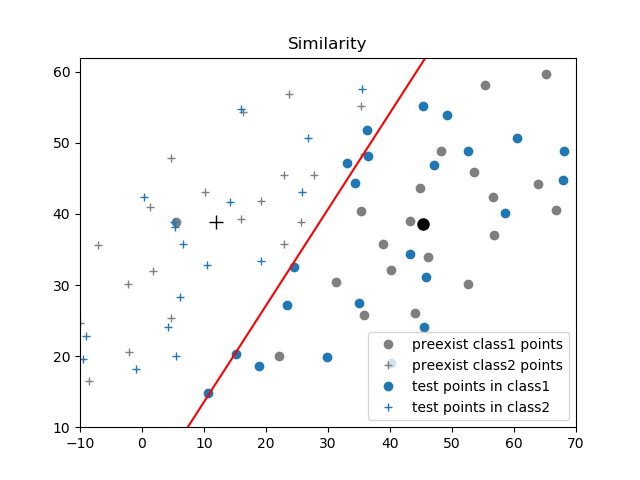
\includegraphics[width=15.0cm, bb=9 9 700 270]{results/SimilarityResultFigureC.png}
   		\hspace{0cm} (e) The result of using Similarity method. (C)
   	\end{minipage}
   \end{tabular}
 \end{figure}

\clearpage
\setcounter{subsection}{1}
\subsection{データセットD}

\begin{table}[htbp]
  \caption{方法別認識正誤表(D)}
  \begin{tabular}{|c||c|c|} \hline
    方法 & 正誤 & 認識率[\%] \\ \hline
    Nearest & TTTTTTTTTTFTTTTTTFTFTTTTTTTTTTTTTTTTTFTT & 90.0 \\\hline
    ユークリッド距離 & TFTTTTTTTTTTTFTTFFTFTTTTTTTTTFTFTTFTTFTT & 77.5 \\\hline
    重み付きユークリッド & TFTTTTTTTTTTTTTTTFTFTTTTTTTTTTTTTTTTTFTT & 90.0\\\hline
    類似度 & TFTTTTTTTTTTTFTTFFTFTTTTTTTTTFTFTTFTTFTT & 77.5\\\hline
  \end{tabular}
\end{table}

 \begin{figure}[hbtp]
   \centering
   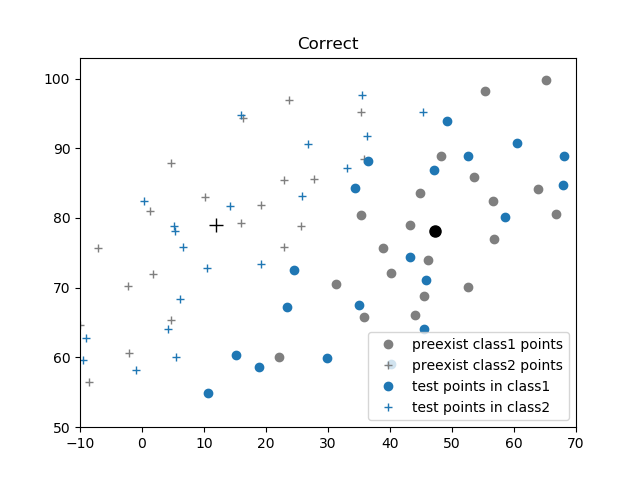
\includegraphics[width=26cm, bb=9 9 700 350]{results/CorrectResultFigureD.png}
   \caption{(a) Correct distribution of test set D.}
 \end{figure}

 \begin{figure}[htbp]
   \centering
   \begin{tabular}{c}
   	\begin{minipage}{0.56\hsize}
   	\centering
   		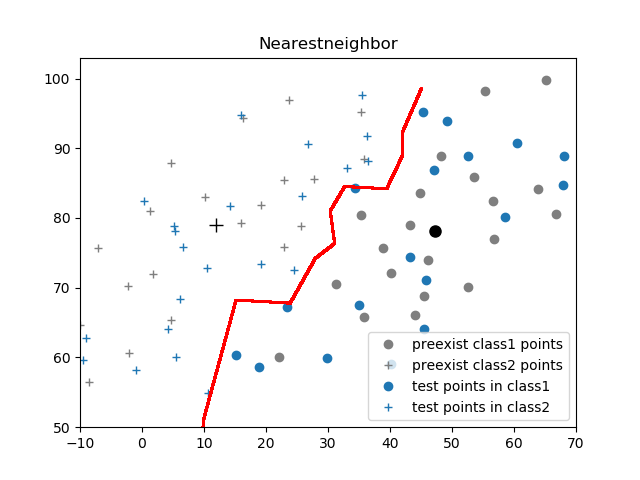
\includegraphics[width=15.0cm, bb=9 9 700 270]{results/NearestneighborResultFigureD.png}
   		\hspace{0cm} (b) The result of using Nearest Neighbor method. (D)
   	\end{minipage}

   	\begin{minipage}{0.5\hsize}
   	\centering
   		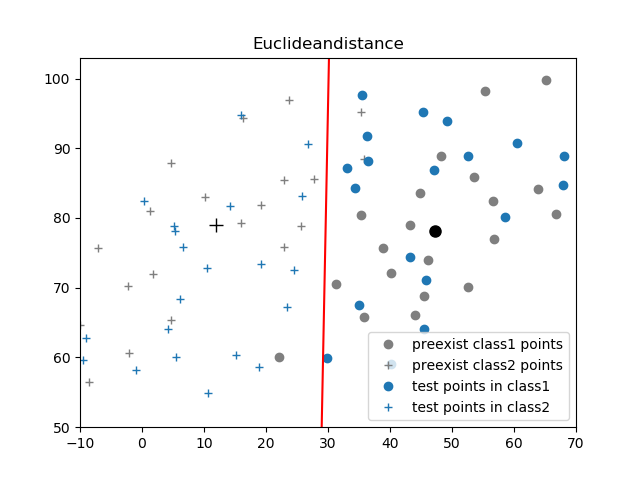
\includegraphics[width=15.0cm, bb=9 9 700 270]{results/EuclideandistanceResultFigureD.png}
   		\hspace{0cm} (b) The result of using EuclideanDistance method.
   	\end{minipage}
   \end{tabular}
 \end{figure}
 \begin{figure}[htbp]
   \centering
   \begin{tabular}{c}
   	\begin{minipage}{0.56\hsize}
   	\centering
   		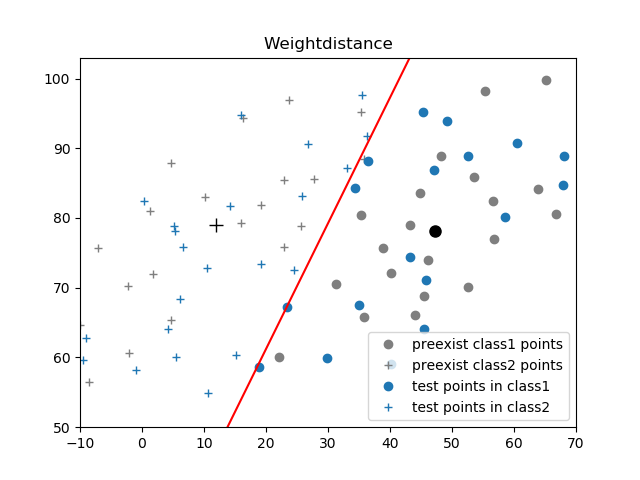
\includegraphics[width=15.0cm, bb=9 9 700 270]{results/WeightdistanceResultFigureD.png}
   		\hspace{0cm} (d) The result of using Weight Euclidean method. (D)
   	\end{minipage}

   	\begin{minipage}{0.5\hsize}
   	\centering
   		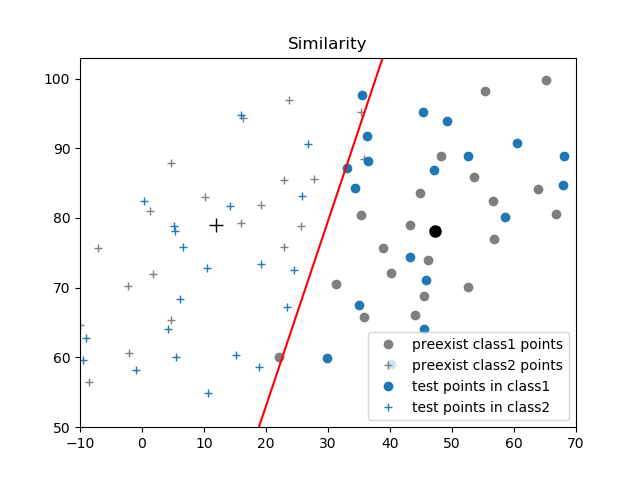
\includegraphics[width=15.0cm, bb=9 9 700 270]{results/SimilarityResultFigureD.png}
   		\hspace{0cm} (e) The result of using Similarity method. (D)
   	\end{minipage}
   \end{tabular}
 \end{figure}

\subsection{(d)}
B, C, Dデータセットの判別結果もセットAと同じような結果が得られた. 結論から言うと, 今回の学習データはクラス間が適度に空白地帯が空いており,
お互い交じり合っている部分も少ない(ノイズが少ない)ためnearest neighbor法はいずれのデータセットにおいても高い認識率を示した.
その他の方法ではクラスデータを無理やり一次関数で分断しようとしているため, 認識率をあげたくても限界があると予想できる. この困難を克服ため
高次方程式で識別境界線を描けるアルゴリズムを作る必要があると考えられる.

\subsection{(e)}
重み付きユークリッド距離法において重みを変えるというのは各軸の重みを変え, 識別線の傾きを変えるということを意味する.
データセットAにおいて重みを(1,5)と(1,20)にした結果を下図5に示す. 明らかのように, y座標がクラス判別に与える影響は(1,20)の方が
遥かに大きいことがわかった.

\begin{figure}[htbp]
  \centering
  \begin{tabular}{c}
   \begin{minipage}{0.56\hsize}
   \centering
     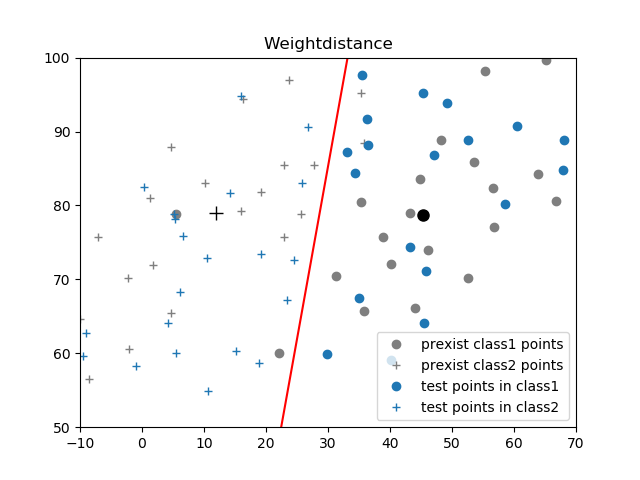
\includegraphics[width=15.0cm, bb=9 9 700 270]{results/WeightdistanceResultFigureA.png}
     \hspace{0cm} (a) Weight (1,5)
   \end{minipage}

   \begin{minipage}{0.5\hsize}
   \centering
     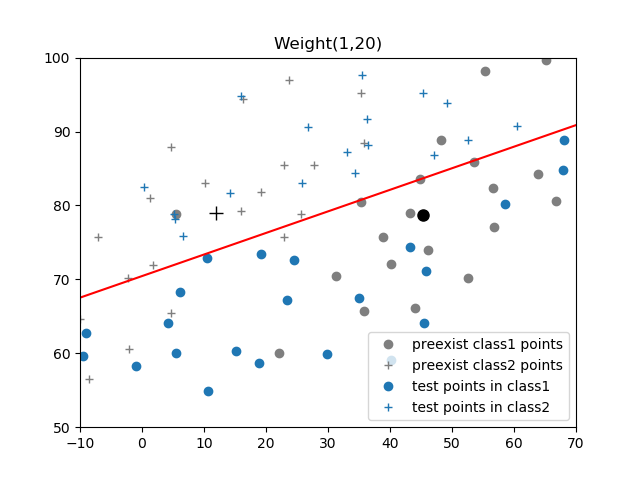
\includegraphics[width=15.0cm, bb=9 9 700 270]{results/Weight(1,20)ResultFigureA.png}
     \hspace{0cm} (b) Weight (1,20)
   \end{minipage}
  \end{tabular}
\end{figure}



\end{document}
